\section{The Editor Aspect}
\label{chap:editor_aspect}

After we have imported all concepts, their contents (properties) and linked them together (child links), it is time to define, what is the visual representation of these concepts.
Without this, we are not able to start using the language inside MPS.
\\

As stated before (Section~\ref{chap:about_editor_aspect}), MPS uses a~cellular system that allows placing concept's properties and children into a~table-like arrangement.
MPS has a~lot of different types of cells that we can use:

\begin{itemize}
	\item Cells for storing values of properties -- the user can enter text inside, which is validated using the type of the property (think XML tag name).

	\item Cells for storing child concepts -- here we can store other parser rule references and build the AST further.

	\item Cells that have static fixed content, such as constant keyword -- we will use these to display literal elements.

	\item Cells that influence the layout, such as indenting.
\end{itemize}

Our import plugin has to create these cells and ideally project all of the concept's elements in there.
\\

A part of this thesis' mission was to explore, whether we can also bring some more value into this import step.
The problem with grammars is that it serves us no aid when it comes to element layout.
The grammar only defines, what the rule breaks up into and which elements (rule references, literals..) are contained inside of each alternative.
Since the layout information is missing, we have only two options, how to tackle this problem:

\begin{itemize}
	\item Get this information from the user by prompting for it somehow.
	\item Keep everything automatized and generate the information using some heuristic.
\end{itemize}

It is a~very hard problem, though since our plugin doesn't really understand the contents of the grammar on some higher level.

\subsection{The Interactive Approach}

Since the layout information is just missing, we decided to ask the user for it.
The first idea on how to tackle this problem was to interactively prompt the user during the import process.
We would somehow select rules that we consider important, and give the user several visual options on how we think this rule might be laid out.
The user would pick one and we would use this information to create the editor aspect.
There are some problems with this, though that led to rejecting this approach.

\subsubsection{Detecting Interesting Rules}

Firstly, we would have to be able to tell, which rules might be worth "discussing" with the user.
\\

The first idea for a~heuristic indicating these "interesting" rules was based on a~number of elements contained in rule's alternative.
For simple rules, which there usually is a~big number present in the grammar, we would skip them.
For complex rules (let's say 5 elements and more), we would ask the user for help with the layout.
The heuristic isn't bad, it would detect complicated rules, such as cycles, branching commands and so on, so it might be a~sufficient, yet simple, solution.
It, however, has some problems --- rules describing a~block of statements are usually very simple, example given being the JavaScript one:

\begin{antlr}
	\parserrule{statementList} : \parserrule{statement}* ;
\end{antlr}

This rule would be skipped by our heuristics since the alternative has only one element, but in most general purpose languages, this is exactly the kind of statement that we would like to adjust, since normally we put each statement on a~separate line.
There are dozens of rules that have this form (method parameters, operands, ...), and we have no means of recognizing that this particular one should be a~vertical list (meaning its elements should be separated by a~new line).
\\

Another heuristic suggestion was detecting pair symbols among alternative's literal elements.
Usually, characters such as braces are a~good indicator of some indenting.
We, however, did not implement any of these heuristics, because, in the end, we decided to abandon the interactive approach completely, as described below in Section~\ref{chap:interactive_approach_evaluation}.
That is why we will not go into more detail here.

\subsubsection{Fixing Rule Layout}

Once we have detected a~rule that might have some interesting layout, we would ask the user to help us with adjusting it.
Consider, for example, the first alternative of the \parserrule{element} rule from the XML language:

\begin{antlr}
	\parserrule{element}  :   \literal{<} \lexerrule{Name} \parserrule{attribute}* \literal{>} \parserrule{content}* \literal{</} \lexerrule{Name} \literal{>} ;
\end{antlr}

Let's say, we would prepare few versions of how we think the layout could look like.
We would present these options to the user and let them choose.
We could ask the user, whether attributes should be spread out horizontally or each on a~new line.
We could and probably would have to do this for each element since the plugin has no real understanding of the content.
We would have to ask for indentation, line breaks etc. because if we were to guess, we would probably guess wrong since there are just too many options.
The user would probably end up finalizing the layout himself.
\\

The other option could be in form of some sophisticated smart dialog, where the user would control the layout by dragging the elements around or position them through some text field.
This would be probably better, but we would be reimplementing already existing functionality that is already present inside MPS.
Again, we are not going into any more detail here, as this approach was rejected because of reasons mentioned below.

\subsubsection{Approach Evaluation}
\label{chap:interactive_approach_evaluation}

The author of this thesis came to a~conclusion that the results of the interactive approach would be most likely quite suboptimal.
It would be hard to recognize rules that are in need of a~refactoring.
Furthermore, when asking for user's help, we would just duplicate the functionality of MPS's built-in projectional editor.
We would hardly mimic all of its functionality and put a~lot of effort into something already existent.
Moreover, our end user is expected to have knowledge of the MPS editor, since he is importing language there.
This means that he probably knows his way around the projectional editor too.
It wouldn't make sense to force the user to learn to work with our own interactive dialog, while in the background, this dialog would be just translating the layout back into the terms of the projectional editor.
Implementing such mechanism would also probably be very complicated.
\\

To put it a~bit differently --- we wouldn't be sparing the user from any manual work, we would be only changing the environment, where this work happens.
We would be shifting it from the MPS projectional editor designer into our interactive dialog.
We would be shifting it from a~fully featured MPS environment, the user probably already knows, into a~feature-wise way poorer environment, the user sees for the first time.
We would be doing this shift for a~price of reimplementing already existing mechanisms.
We would also need to decide, where to draw a~line and which layout features we will cover in our interactive dialog (say line breaks and indenting) and which features we would leave out (code colouring, spacing..).
If we didn't draw this line, we would end up reimplementing the whole MPS projectional editor designer.
Furthermore, for every feature that we would choose to include, we would have to implement special behaviour inside the interactive dialog and then another logic that would translate settings from this dialog into the editor aspect.
And even if we accomplished everything mentioned above, we still believe (and have confirmed that by experimenting) that the language would still need to be adjusted inside the projectional editor designer.
\\

From reasons stated above, we rejected the interactive approach.
From exactly the same reasons, we concluded that any approach that would require user input, would be suboptimal to just leaving the user adjusting the layout inside the MPS editor designer.

\subsection{The Learning Approach}
\label{chap:learning_approach}

Since we have rejected user-input based approaches, we are left with heuristics.
The second approach is more complex and might yield better results.
We have, however, not implemented it to a~stage that would be presentable, as we met some obstacles.
We would like to describe it anyway, so possible follow-up work might take it into consideration.
\\

\subsubsection{Approach Principle}

The learning approach would require the user to, together with the grammar file, supply a~set of valid source files written in the imported language.

\begin{enumerate}
	\item The plugin would automatically generate an ANTLR parser for this language using the ANTLR library, which provides this functionality.

	\item It would alter the code of the generated parser and add some additional functionality, described below.

	\item It would compile the parser into an executable form.

	\item It would use the parser to parse the supplied source code and extract information about the layout of the code.
\end{enumerate}

The benefit of this approach is that the imported language would inherit its code style from the user, as it would learn directly from his code.
The quality of the extracted information would depend on the amount of the code supplied.
So far, this approach sounds very complicated --- extracting layout information sounds like a~difficult problem on its own.
We have, however, found a~simple way, how to mine information very efficiently.
\\

When the ANTLR parser is parsing the code, in its first stage, it reads the input and tries to split it into tokens.
In the second stage, it tries to map the token stream onto parser rules of the language and build an AST.
Earlier, in step 2, we said that we would change the code of the parser.
We would make sure that each parsed token would remember additional information --- the number of the line it appeared on.
This is an easily accessible property of the parser and the ANTLR framework gives us a~lot of room for an adjustment like this.
\\

\noindent
For example, for our \parserrule{element} rule

\begin{antlr}
	\parserrule{element}  :   \literal{<} \lexerrule{Name} \parserrule{attribute}* \literal{>} \parserrule{content}* \literal{</} \lexerrule{Name} \literal{>} ;
\end{antlr}

\noindent
and following source code,

\begin{antlr}
	1   <div>
	2      ... some content ...
	3   </div>
\end{antlr}

\noindent
it would yield something like this:

\begin{antlr}
	TOKEN LINE
	----------
	<       1
	Name    1
	>       1
	\textcolor{gray}{...}
	\textcolor{gray}{// Here, tokens of the content would come}
	\textcolor{gray}{...}
	</      3
	Name    3
	>       3
\end{antlr}

From this, we could clearly derive that there is a~line break between the first closing \textit{greater-than} bracket, the content and then again when the closing tag starts.
Probably, we might also be able to detect indentation, if we would decide to store the column information too, but we haven't explored this possibility.

\subsubsection{Approach Evaluation}

We have started implementing a~proof of concept for this approach, so that we can see, whether it is a~viable solution.
Unfortunately, there were some obstacles, due to which we haven't finished the implementation.
The biggest problem that we have identified, was parser generation.
We found out that even a~small tweaks in the grammar that the user might perform in order to improve the resulting MPS language, can break it enough so that the automatically generated ANTLR parser is not parsing the code correctly.
We talk further about this problem in more detail in Chapter~\ref{chap:breaking_the_parser}.
\\

Other problems that we have identified, were connected to the environment, where it might not be always possible, to perform actions such as parser generation, parser compilation or dynamic loading of the parser.
More problems concerned the algorithm itself, where we would need to be able to match language concepts with all tokens that belong to it.
Mapping the parsed ANTLR AST to the MPS one is a~complex problem that is also connected to parsing any given text source code and importing it inside MPS.
This is considered as an advanced functionality that will probably be subject to a~separate follow-up work.
\\

Because of the overall complexity of this approach and because of reasons stated in Section~\ref{chap:editor_solution}, we have decided to abandon the implementation and only suggest it as a~possible follow-up.
We, however, concluded that this might be a~viable solution for detecting code layout.

\subsection{Our Solution}
\label{chap:editor_solution}

When the author of this thesis worked on the plugin, he noticed that the most tiresome and likely error-prone part of working on the editor aspect is incorporating all concept's properties, children, and constant fields into the editor.
This means a~manual creation of all cells that should appear in the visual representation.
We identified this phase as a~time consuming but also quite straightforward, as it does not require any major thought on user's part.
We have also further noticed that when the plugin would do this heavy lifting, even without layout detection, further adjustments of the editor are very fast since MPS enables doing this very efficiently.
We noticed that even the most obvious way of editor generation, such as plain inlining of all of the cells in a~single row (shown in Figure~\ref{fig:editor_adjustment} on top), might be a~sufficient solution.
In Figure~\ref{fig:editor_adjustment}, we can see an editor adjustment of the \concept{Element{\_}1} concept that can be done in just a~few clicks, but finalizes the editor to its perfect form, better than any heuristics would come up with.
\\

\begin{figure}[ht]
	\centering
	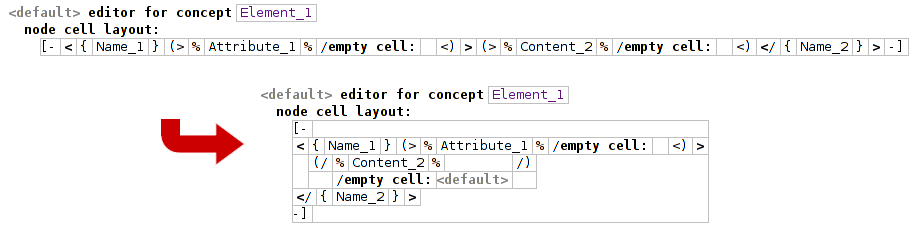
\includegraphics[width=\textwidth]{./img/editor_adjustment.png}
	\caption{Projectional editor adjustment of the Element{\_}1 concept}
	\label{fig:editor_adjustment}
\end{figure}

From these reasons, we concluded that for our cause, it might be sufficient, if the plugin only prepared contents of all editor aspects and the end user would take it from there, reaching optimal results in a~very short time.
We have confirmed this assumption by importing the JavaScript language~\cite{javascript} and manually adjusting all editors that needed it, in a~less than hour time.
We have described this further in Chapter~\ref{chap:examples}.
Further improvements might be a~subject for a~follow-up work, potentially leveraging the second approach, we have described above in Section~\ref{chap:learning_approach}.

